\documentclass[lang=en,11pt,fancy,color=blue]{elegantbook}

\title{Supervised Machine Learning Handbook}
\subtitle{From Intuition to Implementation}
\author{Nishant \& The AI Team}
\institute{IITH Placement Prep}
\date{\today}
\version{1.0}

\usepackage{graphicx}
\graphicspath{{assets/}}

\begin{document}

\maketitle
\tableofcontents

\part{Linear Regression}
\chapter{Simple Linear Regression}
\label{chap:simple_linear_regression}

% ========================================
% SECTION 1: INTRODUCTION
% ========================================
\section{Introduction: What is Regression?}
Imagine you are a college student appearing for campus placements. You notice a pattern among your seniors: those with higher CGPAs tend to get higher salary packages.

\begin{itemize}
    \item \textbf{Student A}: 6.0 CGPA $\rightarrow$ 4 LPA
    \item \textbf{Student B}: 7.0 CGPA $\rightarrow$ 6 LPA
    \item \textbf{Student C}: 9.0 CGPA $\rightarrow$ ?
\end{itemize}

Your intuition tells you that Student C will likely get something higher than 6 LPA, perhaps around 10 LPA. What your brain just did is called \textbf{Regression}. You identified a relationship between an input (CGPA) and an output (Package) and used it to predict a future value.

\begin{definition}
\textbf{Regression}: A supervised learning technique where the goal is to predict a \textbf{continuous} numerical output variable based on one or more input features.
\end{definition}

\begin{definition}
\textbf{Linear Regression}: A specific type of regression where we assume the relationship between the input ($x$) and output ($y$) can be represented by a \textbf{straight line}.
\end{definition}

% ========================================
% SECTION 2: INTUITION
% ========================================
\section{Intuition: The Line of Best Fit}
Let us visualize this concept. Suppose we plot each student as a point on a graph, with CGPA on the X-axis and Package on the Y-axis.

\begin{figure}[htbp]
\centering
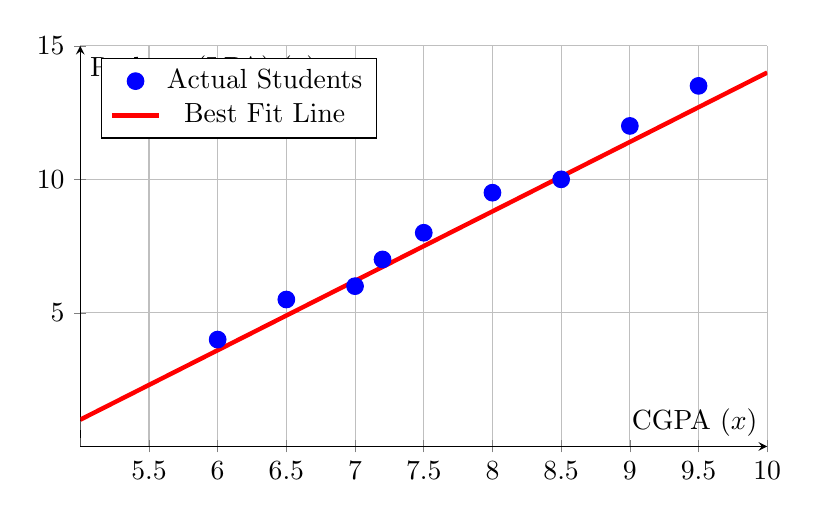
\begin{tikzpicture}
    \begin{axis}[
        xlabel={CGPA ($x$)},
        ylabel={Package (LPA) ($y$)},
        xmin=5, xmax=10,
        ymin=0, ymax=15,
        axis lines=middle,
        grid=major,
        width=0.85\textwidth,
        height=0.55\textwidth,
        legend pos=north west
    ]
    % Data Points
    \addplot[only marks, mark=*, color=blue, mark size=3pt] coordinates {
        (6, 4) (6.5, 5.5) (7, 6) (7.2, 7) (7.5, 8) (8, 9.5) (8.5, 10) (9, 12) (9.5, 13.5)
    };
    \addlegendentry{Actual Students}
    
    % Regression Line
    \addplot[domain=5:10, color=red, ultra thick] {2.6*x - 12};
    \addlegendentry{Best Fit Line}
    
    % Intercept Annotation
    \draw[dashed, gray] (axis cs:5, 0) -- (axis cs:5, 1);
    \node[left] at (axis cs:5, 1) {$c$ (Intercept)};
    \end{axis}
\end{tikzpicture}
\caption{The ``Best Fit Line'' passes through the center of the scattered data points.}
\label{fig:best_fit_intuition}
\end{figure}

The goal of Linear Regression is to find the \textbf{Best Fit Line}. Imagine holding a stick over the scatter plot:
\begin{enumerate}
    \item You move the stick up, down, and rotate it.
    \item Your goal is to make the stick pass \textit{as close as possible} to all the points.
    \item Mathematically, you are minimizing the total ``distance'' (error) between the points and your stick.
\end{enumerate}

% ========================================
% SECTION 3: MATHEMATICAL FORMULATION
% ========================================
\section{Mathematical Formulation}
Every straight line in the world can be written as:
\begin{equation}
    y = mx + c
    \label{eq:line}
\end{equation}
In Machine Learning, we often use slightly different notation ($\beta$ for coefficients):
\begin{equation}
    y = \beta_0 + \beta_1 x
\end{equation}

\begin{itemize}
    \item $y$: The \textbf{Target} (Dependent Variable). This is what we want to predict (e.g., Package).
    \item $x$: The \textbf{Feature} (Independent Variable). This is our input (e.g., CGPA).
    \item $\beta_1$ (or $m$): The \textbf{Slope} or \textbf{Weight}. It tells us how steeply the Package rises with CGPA. A high slope means a small increase in CGPA leads to a huge jump in salary.
    \item $\beta_0$ (or $c$): The \textbf{Intercept} or \textbf{Bias}. This is the baseline value. If CGPA were 0, this would be the predicted package. (Mathematically necessary, though practically, no one has 0 CGPA.)
\end{itemize}

\textbf{The Core Question}: How do we find the optimal values of $m$ and $c$?

% ========================================
% SECTION 4: WORKED EXAMPLE (OLS DERIVATION)
% ========================================
\section{Finding $m$ and $c$: Ordinary Least Squares (OLS)}
This is the heart of Linear Regression. We will derive the formulas step-by-step.

\subsection{Step 1: Define the Error}
For any single data point $i$, the \textbf{error} (or \textbf{residual}) is the difference between the actual value ($y_i$) and the predicted value ($\hat{y}_i$).
\begin{equation}
    \text{Residual}_i = y_i - \hat{y}_i = y_i - (mx_i + c)
\end{equation}

\subsection{Step 2: Define the Loss Function (SSE)}
We cannot simply add up the errors because positive and negative errors cancel each other out.
\textbf{Solution}: Square the errors. This removes negative signs and penalizes large errors more heavily.
\begin{definition}
\textbf{Sum of Squared Errors (SSE)}: The total squared difference between actual and predicted values.
\begin{equation}
    J(m, c) = \sum_{i=1}^{n} (y_i - \hat{y}_i)^2 = \sum_{i=1}^{n} (y_i - mx_i - c)^2
\end{equation}
\end{definition}
\textbf{Goal}: We want to find the values of $m$ and $c$ that \textbf{minimize} $J$.

\subsection{Step 3: Minimize Loss using Calculus}
To find the minimum of a curve, we take the derivative and set it to zero.

\textbf{(A) Derivative with respect to $c$:}
\begin{align}
    \frac{\partial J}{\partial c} &= \sum 2(y_i - mx_i - c)(-1) = 0 \\
    -2 \sum (y_i - mx_i - c) &= 0 \\
    \sum y_i - m \sum x_i - nc &= 0 \\
    c &= \bar{y} - m\bar{x}
\end{align}
Where $\bar{y} = \frac{\sum y_i}{n}$ and $\bar{x} = \frac{\sum x_i}{n}$ are the means.

\textbf{(B) Derivative with respect to $m$:}
After substituting $c$ and simplifying (algebra omitted for brevity), we get:
\begin{equation}
    \boxed{m = \frac{\sum (x_i - \bar{x})(y_i - \bar{y})}{\sum (x_i - \bar{x})^2}}
    \label{eq:ols_m}
\end{equation}
\begin{equation}
    \boxed{c = \bar{y} - m\bar{x}}
    \label{eq:ols_c}
\end{equation}
These are the famous \textbf{OLS formulas}.

% ========================================
% SECTION 5: CODE IMPLEMENTATION
% ========================================
\section{Implementation in Python}
Let us build a Simple Linear Regression model using \texttt{scikit-learn}.

\begin{lstlisting}[language=Python, caption=Simple Linear Regression with Scikit-Learn]
import numpy as np
import matplotlib.pyplot as plt
from sklearn.linear_model import LinearRegression

# =============================================
# STEP 1: Create Dummy Data
# =============================================
np.random.seed(42)  # For reproducibility
# 100 students with CGPA between 5 and 10
X = np.random.uniform(5, 10, 100).reshape(-1, 1)
# Package roughly follows: 2.5 * CGPA - 8 (plus noise)
y = 2.5 * X - 8 + np.random.normal(0, 1.5, (100, 1))

# =============================================
# STEP 2: Train the Model
# =============================================
model = LinearRegression()
model.fit(X, y)  # The model calculates 'm' and 'c' using OLS

# =============================================
# STEP 3: Check Learned Parameters
# =============================================
print(f"Slope (m): {model.coef_[0][0]:.4f}")       # Expected: ~2.5
print(f"Intercept (c): {model.intercept_[0]:.4f}") # Expected: ~-8

# =============================================
# STEP 4: Visualize the Result
# =============================================
plt.figure(figsize=(10, 6))
plt.scatter(X, y, color='blue', alpha=0.6, label='Actual Data')
plt.plot(X, model.predict(X), color='red', linewidth=2, label='Best Fit Line')
plt.xlabel('CGPA')
plt.ylabel('Package (LPA)')
plt.title('Simple Linear Regression')
plt.legend()
plt.grid(True)
plt.show()
\end{lstlisting}

% ========================================
% SECTION 6: VISUALIZATION (Already in Section 2)
% ========================================
% (Visualization is integrated into Section 2 with TikZ)

% ========================================
% SECTION 7: SUMMARY / KEY TAKEAWAYS
% ========================================
\section{Key Takeaways}
\begin{enumerate}
    \item \textbf{Assumption}: Linear Regression assumes the data follows a straight line ($y = mx + c$).
    \item \textbf{Goal}: Find the line that minimizes the Sum of Squared Errors (SSE).
    \item \textbf{Parameters}: The model learns two things:
    \begin{itemize}
        \item \textbf{Slope ($m$)}: The strength of the relationship.
        \item \textbf{Intercept ($c$)}: The baseline value.
    \end{itemize}
    \item \textbf{Method}: Ordinary Least Squares (OLS) provides a closed-form formula for $m$ and $c$.
\end{enumerate}

% ========================================
% SECTION 8: HOTS QUESTIONS
% ========================================
\section{HOTS: Interview Questions}
\textbf{Q1: What are the key assumptions of Linear Regression?}
\begin{itemize}
    \item \textbf{Linearity}: The relationship between $X$ and $Y$ is linear.
    \item \textbf{Independence}: Observations are independent.
    \item \textbf{Homoscedasticity}: Constant variance of errors.
    \item \textbf{Normality}: Residuals should be normally distributed.
    \item \textbf{No Multicollinearity}: Features should not be highly correlated with each other.
\end{itemize}

\textbf{Q2: Why do we square the residuals instead of using absolute values?}
\begin{itemize}
    \item Squaring removes negative signs, ensuring errors do not cancel out.
    \item Squaring penalizes larger errors more heavily.
    \item The squared function is \textbf{smooth} (differentiable everywhere), which is essential for optimization algorithms like Gradient Descent.
    \item The absolute value function $|x|$ has a sharp ``V'' shape at zero, making it non-differentiable at that point.
\end{itemize}

\textbf{Q3: Is OLS suitable for very large datasets?}
\begin{itemize}
    \item Not always. OLS involves matrix inversion ($(X^TX)^{-1}$), which has a time complexity of $O(n^3)$.
    \item For massive datasets, \textbf{Gradient Descent} is preferred as it iteratively approximates the solution with lower memory usage.
\end{itemize}

\chapter{Gradient Descent}

\section{Introduction}
In Chapter 1, we found the best fit line using the \textbf{OLS (Ordinary Least Squares)} formula. It gave us the exact answer instantly. So why do we need another method?

\begin{itemize}
    \item \textbf{Computational Cost}: OLS involves matrix inversion, which becomes extremely slow ($O(n^3)$) for very large datasets with many features.
    \item \textbf{Memory}: OLS requires loading the entire dataset into memory to perform matrix operations.
\end{itemize}

\textbf{Gradient Descent} is an iterative optimization algorithm that finds the minimum of a function step-by-step. It is the backbone of modern Machine Learning and Deep Learning.

\section{Intuition: The Hiker in the Valley}
Imagine you are blindfolded at the top of a mountain (High Loss). Your goal is to reach the lowest point in the valley (Minimum Loss).

\begin{enumerate}
    \item \textbf{Feel the slope}: You test the ground with your feet to see which way is "down".
    \item \textbf{Take a step}: You take a small step in the steepest downward direction.
    \item \textbf{Repeat}: You keep doing this until the ground becomes flat (Slope = 0). You have reached the bottom.
\end{enumerate}

\begin{figure}[htbp]
    \centering
    \includegraphics[width=0.6\textwidth]{gradient_descent_bowl.png}
    \caption{Gradient Descent descending towards the global minimum.}
\end{figure}

\section{Mathematical Formulation}

We want to find values for $m$ (slope) and $c$ (intercept) that minimize the Cost Function $J(m,c) = \sum (y_i - (mx_i+c))^2$.

\subsection{The Update Rule}
At each step, we update our weights ($m, c$) by moving against the gradient.
\begin{equation}
    \theta_{new} = \theta_{old} - \alpha \times \frac{\partial J}{\partial \theta}
\end{equation}
Where:
\begin{itemize}
    \item $\theta$: The parameter we are updating ($m$ or $c$).
    \item $\alpha$ (Alpha): \textbf{Learning Rate}. The size of the step we take.
    \item $\frac{\partial J}{\partial \theta}$: The Gradient (Slope).
\end{itemize}

For Linear Regression, the gradients are:
\[ \frac{\partial J}{\partial m} = -2 \sum x_i(y_i - \hat{y}_i) \quad ; \quad \frac{\partial J}{\partial c} = -2 \sum (y_i - \hat{y}_i) \]

\section{The Role of Learning Rate ($\alpha$)}
\begin{enumerate}
    \item \textbf{Too Small}: The algorithm takes tiny steps. It will eventually reach the minimum, but it will take forever (slow convergence).
    \item \textbf{Too Large}: The algorithm takes giant leaps. It might step \textit{over} the valley and reach the other side, potentially diverging and never finding the minimum.
    \item \textbf{Just Right}: A balanced rate ensures smooth and efficient convergence.
\end{enumerate}

\section{Types of Gradient Descent}
Depending on how much data we use to calculate the gradient for one step, there are three variants.

\subsection{Batch Gradient Descent}
\begin{itemize}
    \item \textbf{Method}: Uses \textbf{ALL} training examples to calculate the gradient for a single update.
    \item \textbf{Pros}: Stable convergence; theoretically guaranteed to find the global minimum for convex functions.
    \item \textbf{Cons}: Very slow per iteration for large datasets; high memory usage.
    \item \textbf{Analogy}: Asking \textit{every single voter} before making a policy change.
\end{itemize}

\subsection{Stochastic Gradient Descent (SGD)}
\begin{itemize}
    \item \textbf{Method}: Uses \textbf{ONE} random training example to calculate the gradient and update weights.
    \item \textbf{Pros}: Extremely fast iterations; good for massive data; helps escape local minima in non-convex problems (due to noise).
    \item \textbf{Cons}: Noisy convergence (zig-zag path); never settles exactly at the minimum.
    \item \textbf{Analogy}: Asking \textit{one random person} on the street and changing policy immediately.
\end{itemize}

\begin{figure}[htbp]
    \centering
    \includegraphics[width=0.7\textwidth]{batch_vs_sgd_contour.png}
    \caption{Batch GD (smooth) vs SGD (noisy) convergence paths.}
\end{figure}

\subsection{Mini-Batch Gradient Descent}
\begin{itemize}
    \item \textbf{Method}: Uses a small \textbf{Batch} (e.g., 32, 64) of examples for one update.
    \item \textbf{Verdict}: The sweet spot. Faster than Batch, more stable than SGD. The industry standard for Deep Learning.
\end{itemize}

\section{Implementation from Scratch (Batch GD)}

\begin{lstlisting}[language=Python, caption=Batch Gradient Descent]
class BatchGD:
    def __init__(self, learning_rate=0.01, epochs=100):
        self.m = 1 # Random initialization
        self.c = 0
        self.lr = learning_rate
        self.epochs = epochs
        
    def fit(self, X, y):
        n = len(X)
        for i in range(self.epochs):
            # Calculate predictions for ALL data
            y_pred = self.m * X + self.c
            
            # Calculate Gradients (Vectorized)
            grad_m = -2 * np.sum((y - y_pred) * X) / n
            grad_c = -2 * np.sum(y - y_pred) / n
            
            # Update Weights
            self.m = self.m - (self.lr * grad_m)
            self.c = self.c - (self.lr * grad_c)
\end{lstlisting}

\section{Interview Questions}

\begin{enumerate}
    \item \textbf{What is the difference between Batch and Stochastic Gradient Descent?}
    \newline \textit{Answer:} Batch GD uses the entire dataset for one update (stable but slow). SGD uses a single random point for one update (fast but noisy).
    
    \item \textbf{What happens if the Learning Rate is too large?}
    \newline \textit{Answer:} The algorithm might overshoot the minimum, bouncing back and forth with increasing error, eventually causing the parameters to diverge (go to infinity).
    
    \item \textbf{Why do we refer to Linear Regression's Loss Function as "Convex"?}
    \newline \textit{Answer:} A convex function is shaped like a bowl (U-shape) and has only one Global Minimum. This guarantees that Gradient Descent will always converge to the best possible solution (unlike Neural Networks which have Local Minima).
    
    \item \textbf{How does Vectorization speed up Gradient Descent?}
    \newline \textit{Answer:} Vectorization allows us to perform mathematical operations on entire arrays at once using SIMD (Single Instruction, Multiple Data) processing, which is much faster than looping through data points one by one in Python.
\end{enumerate}

\chapter{Multiple Linear Regression \& Polynomials}

\section{Introduction}
In the real world, an outcome is rarely dependent on just one factor.
\begin{itemize}
    \item \textbf{Simple LR}: CGPA $\rightarrow$ Package.
    \item \textbf{Multiple LR}: CGPA + Projects + Communication Skills $\rightarrow$ Package.
\end{itemize}

\begin{definition}{Multiple Linear Regression}
    A statistical technique that uses several explanatory variables ($x_1, x_2, \dots, x_n$) to predict the outcome of a response variable ($y$).
\end{definition}

\section{Geometric Intuition}
\begin{itemize}
    \item \textbf{1 Feature}: A Line in 2D space.
    \item \textbf{2 Features}: A \textbf{Plane} in 3D space.
    \item \textbf{n Features}: A \textbf{Hyperplane} in ($n+1$)-dimensional space.
\end{itemize}

\begin{figure}[htbp]
    \centering
    \includegraphics[width=0.7\textwidth]{multiple_lr_plane.png}
    \caption{The Hyperplane fitting the data points in 3D space.}
\end{figure}

\section{Mathematical Formulation}
The equation becomes:
\[ y = \beta_0 + \beta_1 x_1 + \beta_2 x_2 + \dots + \beta_n x_n + \epsilon \]

\subsection{Matrix Notation}
To solve this efficiently, we use Linear Algebra.
\begin{itemize}
    \item $Y$: Vector of targets $(n \times 1)$.
    \item $X$: Matrix of features $(n \times (m+1))$. We add a column of 1s for the intercept $\beta_0$.
    \item $\beta$: Vector of coefficients.
\end{itemize}

\[ Y = X\beta \]

The solution for $\beta$ that minimizes the squared error is given by the \textbf{Normal Equation}:

\begin{equation}
    \hat{\beta} = (X^T X)^{-1} X^T Y
\end{equation}

\section{Adjusted R2 Score}
When we add more features to a model, the standard $R^2$ score \textbf{never decreases}, even if the new feature is completely useless (random noise). This gives a false sense of improvement.

\textbf{Adjusted $R^2$} fixes this by penalizing the model for adding unnecessary features.

\begin{equation}
    R^2_{adj} = 1 - \frac{(1-R^2)(n-1)}{n-1-k}
\end{equation}
Where $n$ is the number of samples and $k$ is the number of features.
\begin{itemize}
    \item If a useful feature is added: $R^2 \uparrow$ significantly, so $R^2_{adj} \uparrow$.
    \item If a useless feature is added: $R^2$ stays same, but penalty ($k$) increases, so $R^2_{adj} \downarrow$.
\end{itemize}

\section{Polynomial Regression}
What if the data is not linear? (e.g., a parabolic curve). A straight line will \textbf{Underfit} (High Bias).

The trick is to \textbf{generate new features} by raising existing ones to powers.
\[ y = \beta_0 + \beta_1 x + \beta_2 x^2 \]

\begin{remark}
    This is still considered \textbf{Linear Regression} because it is linear in terms of the coefficients $\beta$. Let $x^2 = z$, then $y = \beta_0 + \beta_1 x + \beta_2 z$, which is standard Multiple Regression.
\end{remark}

\begin{figure}[htbp]
    \centering
    \includegraphics[width=0.8\textwidth]{polynomial_degrees_comparison.png}
    \caption{Degree 1 (Underfit), Degree 2 (Good Fit), Degree 20 (Overfit).}
\end{figure}

\section{Python Implementation (Polynomial)}

\begin{lstlisting}[language=Python, caption=Polynomial Regression Pipeline]
from sklearn.preprocessing import PolynomialFeatures
from sklearn.linear_model import LinearRegression
from sklearn.pipeline import Pipeline

# 1. Create a Pipeline
# It first transforms data (x -> x, x^2), then fits Linear Regression
pipe = Pipeline([
    ('poly', PolynomialFeatures(degree=2)),
    ('model', LinearRegression())
])

# 2. Fit and Predict
pipe.fit(X_train, y_train)
y_pred = pipe.predict(X_test)
\end{lstlisting}

\section{Interview Questions}

\begin{enumerate}
    \item \textbf{Why is Polynomial Regression considered a Linear Model?}
    \newline \textit{Answer:} Because the relationship between the coefficients ($\beta$) and the target ($y$) remains linear. We are only transforming the input features, not the parameters.
    
    \item \textbf{What is the "Curse of Dimensionality"?}
    \newline \textit{Answer:} As the number of features increases, the amount of data required to generalize accurately grows exponentially. In high dimensions, data becomes sparse, and distance metrics (like Euclidean) become meaningless.
    
    \item \textbf{When should you use Lasso over Ridge?}
    \newline \textit{Answer:} Use Lasso (L1) when you suspect that many features are irrelevant. Lasso tends to drive coefficients of useless features to exactly zero, effectively performing feature selection. Ridge (L2) shrinks them but keeps them non-zero.
    
    \item \textbf{What happens if $(X^T X)$ is not invertible in the Normal Equation?}
    \newline \textit{Answer:} This occurs if there is perfect multicollinearity (features are linearly dependent) or if $n < k$ (more features than samples). To fix it, we can remove correlated features or use Regularization.
\end{enumerate}

\chapter{Regularization}

\section{The Bias-Variance Tradeoff}
Before we fix a model, we must understand how it fails.
\begin{itemize}
    \item \textbf{Bias (Underfitting)}: The model is too simple. It fails to capture the underlying trend. (e.g., Fitting a straight line to a curve).
    \item \textbf{Variance (Overfitting)}: The model is too complex. It memorizes the noise in the training data. (e.g., A wiggly line connecting every dot).
\end{itemize}

\begin{figure}[htbp]
    \centering
    \includegraphics[width=0.9\textwidth]{bias_variance_tradeoff.png}
    \caption{Underfitting (High Bias) vs Overfitting (High Variance).}
\end{figure}

\begin{remark}
    \textbf{Regularization} is the technique of adding a "Penalty" to the Loss Function to discourage the model from becoming too complex (having large coefficients).
\end{remark}

\section{Ridge Regression (L2 Regularization)}
Ridge adds a penalty equal to the \textbf{square of the magnitude} of coefficients.

\begin{equation}
    J(\beta) = \text{MSE} + \lambda \sum_{j=1}^{p} \beta_j^2
\end{equation}

\begin{itemize}
    \item As $\lambda$ increases, the coefficients ($\beta$) shrink towards zero.
    \item \textbf{Property}: Coefficients become very small but \textbf{never exactly zero}.
    \item \textbf{Use Case}: Preventing overfitting when all features are somewhat important. Handing Multicollinearity.
\end{itemize}

\begin{figure}[htbp]
    \centering
    \includegraphics[width=0.6\textwidth]{ridge_lambda_error_curve.png}
    \caption{As $\lambda$ increases, Variance decreases but Bias increases.}
\end{figure}

\section{Lasso Regression (L1 Regularization)}
Lasso adds a penalty equal to the \textbf{absolute value} of coefficients.

\begin{equation}
    J(\beta) = \text{MSE} + \lambda \sum_{j=1}^{p} |\beta_j|
\end{equation}

\begin{itemize}
    \item \textbf{Feature Selection}: Lasso tends to force coefficients of useless features to become \textbf{Exactly Zero}.
    \item \textbf{Use Case}: Sparse models; when you suspect many features are irrelevant.
\end{itemize}

\begin{figure}[htbp]
    \centering
    \includegraphics[width=0.7\textwidth]{lasso_vs_ridge_coef_behavior.png}
    \caption{Ridge shrinks asymptotically; Lasso hits zero sharply.}
\end{figure}

\section{Elastic Net}
Combines both L1 and L2 penalties.
\[ J(\beta) = \text{MSE} + \lambda_1 \sum |\beta_j| + \lambda_2 \sum \beta_j^2 \]
\begin{itemize}
    \item Used when we want feature selection (Lasso) but also need stability (Ridge) for correlated features.
\end{itemize}

\section{Python Implementation}

\begin{lstlisting}[language=Python, caption=Regularization in Scikit-Learn]
from sklearn.linear_model import Ridge, Lasso, ElasticNet
from sklearn.preprocessing import StandardScaler

# Standardization is MANDATORY for Regularization
scaler = StandardScaler()
X_scaled = scaler.fit_transform(X)

# Ridge
ridge = Ridge(alpha=1.0)
ridge.fit(X_scaled, y)

# Lasso
lasso = Lasso(alpha=0.1)
lasso.fit(X_scaled, y)
print(f"Zeroed Features: {np.sum(lasso.coef_ == 0)}")

# ElasticNet
enet = ElasticNet(alpha=0.1, l1_ratio=0.5)
enet.fit(X_scaled, y)
\end{lstlisting}

\section{Interview Questions}

\begin{enumerate}
    \item \textbf{Why does Lasso select features (set coefficients to 0) while Ridge does not?}
    \newline \textit{Answer:} Geometrically, the L1 constraint ($|\beta_1| + |\beta_2| \le C$) forms a diamond shape with corners on the axes. The Loss function's contours are likely to touch the diamond at these corners (where one coefficient is 0). The L2 constraint ($\beta_1^2 + \beta_2^2 \le C$) forms a circle, which the contours usually touch at a non-zero point.
    
    \item \textbf{Can we use Regularization without Feature Scaling?}
    \newline \textit{Answer:} \textbf{No.} Regularization penalties depend on the magnitude of coefficients. If one feature has huge values (e.g., Salary) and another small (e.g., Age), the coefficients will be on different scales. The penalty term will unfairly target the feature with smaller coefficients (which might need larger weights to compensate). Scaling ensures fair penalization.
    
    \item \textbf{What is the Bias-Variance Tradeoff relative to $\lambda$?}
    \newline \textit{Answer:}
    \begin{itemize}
        \item Low $\lambda$: Complex model $\rightarrow$ High Variance, Low Bias (Overfitting).
        \item High $\lambda$: Simple model $\rightarrow$ Low Variance, High Bias (Underfitting).
    \end{itemize}
\end{enumerate}


\part{Logistic Regression}
\chapter{Logistic Regression: Intuition}

\section{Introduction}

Despite its name containing "Regression", \textbf{Logistic Regression} is a \textbf{Classification} algorithm. It is used to predict discrete categories (e.g., Spam or Not Spam, Tumor Malignant or Benign).

\begin{definition}{Logistic Regression}
    A supervised learning algorithm that predicts the probability of a target variable belonging to a particular class. It uses the logistic (sigmoid) function to map predictions to values between 0 and 1.
\end{definition}

\section{Geometric Intuition}

Imagine we have two classes of points on a 2D plane: Blue (Class 0) and Green (Class 1).
Our goal is to find a \textbf{Line} (in 2D) or \textbf{Hyperplane} (in 3D+) that best separates these two classes.

The equation of the boundary is:
\[ z = w_1 x_1 + w_2 x_2 + b \]

\begin{itemize}
    \item If $z > 0$: We predict \textbf{Positive Class}.
    \item If $z < 0$: We predict \textbf{Negative Class}.
\end{itemize}

\begin{figure}[htbp]
    \centering
    \includegraphics[width=0.6\textwidth]{log_reg_linear_boundary.png}
    \caption{A linear decision boundary separating two classes.}
\end{figure}

\section{The Perceptron Trick (Push and Pull)}
Before modern Logistic Regression, there was the Perceptron. Its learning logic gives us great intuition.

\subsection{The Algorithm}
\begin{enumerate}
    \item Start with a random line.
    \item Pick a random point.
    \item If it is \textbf{Misclassified}, move the line to fix it.
    \item Repeat.
\end{enumerate}

\subsection{Push and Pull Logic}
\begin{itemize}
    \item \textbf{Case 1: Positive point in Negative Region}.
    \newline The point says: "I should be positive!". It \textbf{pulls} the line towards itself so it crosses over into the positive side.
    \item \textbf{Case 2: Negative point in Positive Region}.
    \newline The point says: "I should be negative!". It \textbf{pushes} the line away.
\end{itemize}

\begin{figure}[htbp]
    \centering
    \includegraphics[width=0.7\textwidth]{perceptron_push_pull_vectors.png}
    \caption{Visualizing how misclassified points update the line weights.}
\end{figure}

\subsection{The Flaw: Lack of Conviction}
The Perceptron stops the moment all points are classified correctly.
\begin{itemize}
    \item It doesn't care if a point is \textit{barely} correct (distance = $0.0001$) or \textit{very} confident (distance = $100$).
    \item \textbf{Result}: The boundary might end up too close to the data points (Low Margin), leading to poor generalization.
\end{itemize}

\section{The Solution: Sigmoid Function}
To fix this, we need a method that considers \textbf{Distance} (how far a point is from the line) and converts it into a \textbf{Probability} (0 to 1).

We typically use the \textbf{Sigmoid Function} $\sigma(z)$:

\begin{equation}
    \sigma(z) = \frac{1}{1 + e^{-z}}
\end{equation}

\begin{figure}[htbp]
    \centering
    \includegraphics[width=0.6\textwidth]{sigmoid_curve_annotated.png}
    \caption{The Sigmoid function squashes values between 0 and 1.}
\end{figure}

\begin{itemize}
    \item If $z = 0$ (on the line) $\rightarrow \sigma(z) = 0.5$ (Unsure).
    \item If $z \to +\infty$ (far positive) $\rightarrow \sigma(z) \to 1$ (Confident Positive).
    \item If $z \to -\infty$ (far negative) $\rightarrow \sigma(z) \to 0$ (Confident Negative).
\end{itemize}

By using Sigmoid, we transform our "Line" into a continuous "Probability Landscape". Now, even correctly classified points can push the line further away to increase confidence (probability).

\section{Interview Questions}

\begin{enumerate}
    \item \textbf{Is Logistic Regression a Linear model?}
    \newline \textit{Answer:} \textbf{Yes.} Even though the Sigmoid function is non-linear, the decision boundary it finds ($w^Tx + b = 0$) is linear (a straight line or hyperplane).
    
    \item \textbf{Why do we use Sigmoid instead of a Step Function?}
    \newline \textit{Answer:} The Step Function gives a hard 0 or 1 output, which has a derivative of 0 everywhere (except at the jump where it's undefined). This makes Gradient Descent impossible. The Sigmoid function provides a smooth, differentiable gradient, allowing us to optimize the weights.
    
    \item \textbf{Can Logistic Regression solve non-linear problems?}
    \newline \textit{Answer:} Not by itself. Standard Logistic Regression can only find a linear boundary. However, like Polynomial Regression, we can use \textbf{Feature Engineering} (adding $x^2, x^3$ terms) to create non-linear boundaries.
\end{enumerate}

\chapter{The Math of Classification}

\section{Why not Mean Squared Error (MSE)?}
In Linear Regression, we used MSE as the Loss Function. Can we use it here?
\[ J = \frac{1}{n} \sum (y - \sigma(z))^2 \]

\textbf{No.} Because the Sigmoid function is non-linear, squaring it creates a \textbf{Non-Convex} error surface with many local minima. Gradient Descent is not guaranteed to find the global minimum.

\section{Maximum Likelihood Estimation (MLE)}
Instead of minimizing error, we want to \textbf{Maximize Likelihood}.
We want to find weights $w$ such that the probability of predicting the correct class is maximized for all data points.

\[ L = \prod_{i=1}^{n} P(y_i | x_i; w) \]

Since multiplying many probabilities (decimals $<1$) leads to arithmetic underflow (numbers becoming $0.000\dots$), we take the \textbf{Logarithm} of the Likelihood. And since we want a \textit{Loss} function to \textit{minimize}, we take the negative.

\section{Log Loss (Binary Cross Entropy)}
The cost function for a single example is:
\begin{equation}
    Cost(\hat{y}, y) = - [ y \log(\hat{y}) + (1-y) \log(1-\hat{y}) ]
\end{equation}

\begin{itemize}
    \item \textbf{If $y=1$}: Loss $= - \log(\hat{y})$. We want $\hat{y} \approx 1$ (Loss $\approx 0$).
    \item \textbf{If $y=0$}: Loss $= - \log(1 - \hat{y})$. We want $\hat{y} \approx 0$ (Loss $\approx 0$).
\end{itemize}

\section{Gradient Descent Derivation}
Since there is no "Closed Form" solution (like OLS) due to the non-linearity, we \textbf{must} use Gradient Descent.

We need $\frac{\partial J}{\partial w}$. Using the Chain Rule:
\[ \frac{\partial J}{\partial w} = \frac{\partial J}{\partial \hat{y}} \cdot \frac{\partial \hat{y}}{\partial z} \cdot \frac{\partial z}{\partial w} \]

\begin{enumerate}
    \item \textbf{Derivative of Loss}: $\frac{\partial J}{\partial \hat{y}} = \frac{\hat{y} - y}{\hat{y}(1-\hat{y})}$
    \item \textbf{Derivative of Sigmoid}: $\frac{\partial \hat{y}}{\partial z} = \hat{y}(1-\hat{y})$
    \item \textbf{Derivative of Linear func}: $\frac{\partial z}{\partial w} = x$
\end{enumerate}

\textbf{The Magic Cancellation}:
\[ \frac{\partial J}{\partial w} = \left( \frac{\hat{y} - y}{\hat{y}(1-\hat{y})} \right) \cdot (\hat{y}(1-\hat{y})) \cdot x \]
\[ \frac{\partial J}{\partial w} = (\hat{y} - y)x \]

\begin{remark}
    \textbf{Surprise!} The gradient update rule for Logistic Regression is \textbf{identical} to Linear Regression:
    \[ w_{new} = w_{old} - \alpha (\hat{y} - y)x \]
    The only difference is that $\hat{y}$ here is the Sigmoid probability, whereas in Linear Regression, it was just $mx+c$.
\end{remark}

\section{Python Implementation (From Scratch)}

\begin{lstlisting}[language=Python, caption=Logistic Regression from Scratch]
class LogisticRegression:
    def __init__(self, lr=0.01, epochs=1000):
        self.lr = lr
        self.epochs = epochs
        self.weights = None
        self.bias = 0
        
    def sigmoid(self, z):
        return 1 / (1 + np.exp(-z))
        
    def fit(self, X, y):
        n_samples, n_features = X.shape
        self.weights = np.zeros(n_features)
        
        for _ in range(self.epochs):
            # Forward
            linear_model = np.dot(X, self.weights) + self.bias
            y_pred = self.sigmoid(linear_model)
            
            # Gradient
            dw = (1 / n_samples) * np.dot(X.T, (y_pred - y))
            db = (1 / n_samples) * np.sum(y_pred - y)
            
            # Update
            self.weights -= self.lr * dw
            self.bias -= self.lr * db
            
    def predict(self, X):
        linear_model = np.dot(X, self.weights) + self.bias
        y_pred = self.sigmoid(linear_model)
        return [1 if i > 0.5 else 0 for i in y_pred]
\end{lstlisting}

\chapter{Metrics \& Evaluation}

How do we measure if our classifier is "good"?
Unlike Regression (where we check "how close" the prediction is), Classification is often about "Right or Wrong" ... or is it?

\section{Confusion Matrix}
A 2x2 table showing the breakdown of predictions.

\begin{table}[htbp]
    \centering
    \begin{tabular}{|c|c|c|}
        \hline
         & \textbf{Predicted Positive (1)} & \textbf{Predicted Negative (0)} \\
        \hline
        \textbf{Actual Positive (1)} & \textbf{TP} (True Positive) & \textbf{FN} (False Negative) \\
        \hline
        \textbf{Actual Negative (0)} & \textbf{FP} (False Positive) & \textbf{TN} (True Negative) \\
        \hline
    \end{tabular}
    \caption{Confusion Matrix}
\end{table}

\begin{itemize}
    \item \textbf{Type I Error (FP)}: False Alarm. (e.g., Man told he is pregnant).
    \item \textbf{Type II Error (FN)}: Missed Opportunity. (e.g., Pregnant woman told she is not).
\end{itemize}

\section{Accuracy: The Trap}
\[ \text{Accuracy} = \frac{TP + TN}{\text{Total}} \]
\textbf{Why it fails}: Imagine a dataset with 990 healthy people and 10 cancer patients. If a model predicts "Healthy" for everyone, it achieves \textbf{99\% Accuracy}. But it is useless because it caught 0 cancer cases. This is the \textbf{Imbalanced Data Trap}.

\section{Precision and Recall}
To examine performance more deeply, we ask two specific questions.

\subsection{Precision (Quality)}
"Out of all points predicted as Positive, how many are actually Positive?"
\[ \text{Precision} = \frac{TP}{TP + FP} \]
\begin{itemize}
    \item \textbf{Focus}: Minimize False Positives.
    \item \textbf{Use Case}: \textbf{Spam Filter}. You don't want to classify an important email as Spam (FP). You'd rather let a few Spam emails through (FN).
\end{itemize}

\subsection{Recall (Quantity)}
"Out of all actual Positives, how many did we find?"
\[ \text{Recall} = \frac{TP}{TP + FN} \]
\begin{itemize}
    \item \textbf{Focus}: Minimize False Negatives.
    \item \textbf{Use Case}: \textbf{Cancer Detection}. You don't want to tell a sick patient they are healthy (FN). You'd rather run tests on a healthy person (FP).
\end{itemize}

\section{F1 Score}
The Harmonic Mean of Precision and Recall.
\[ \text{F1} = 2 \times \frac{P \times R}{P + R} \]
Use this when you need a balance (e.g., Cat vs Dog classifier) or when comparing models on imbalanced data.

\section{ROC - AUC Curve}
The \textbf{Receiver Operating Characteristic (ROC)} curve plots the performance at \textbf{all classification thresholds} (0 to 1).

\begin{itemize}
    \item \textbf{X-axis}: False Positive Rate (FPR) = $FP / (FP+TN)$
    \item \textbf{Y-axis}: True Positive Rate (Recall) = $TP / (TP+FN)$
\end{itemize}

\textbf{AUC (Area Under Curve)}:
\begin{itemize}
    \item \textbf{AUC = 1.0}: Perfect Classifier.
    \item \textbf{AUC = 0.5}: Random Guessing (Diagonal Line).
    \item \textbf{AUC < 0.5}: Worse than random.
\end{itemize}

\section{Python Implementation}

\begin{lstlisting}[language=Python, caption=Classification Report]
from sklearn.metrics import classification_report, confusion_matrix, roc_auc_score

# 1. Confusion Matrix
print(confusion_matrix(y_true, y_pred))

# 2. Detailed Report (Precision, Recall, F1)
print(classification_report(y_true, y_pred))

# 3. ROC-AUC (Requires probabilities, not class labels)
# Use predict_proba to get probability of Positive Class (col 1)
y_prob = model.predict_proba(X_test)[:, 1]
print("AUC Score:", roc_auc_score(y_true, y_prob))
\end{lstlisting}

\section{Interview Questions}

\begin{enumerate}
    \item \textbf{Precision vs Recall: Which is more important?}
    \newline \textit{Answer:} It depends on the cost of errors. If False Positives are expensive (Spam Filter), prioritize Precision. If False Negatives are expensive (Medical Diagnosis), prioritize Recall.
    
    \item \textbf{Why use F1 Score instead of Arithmetic Mean?}
    \newline \textit{Answer:} The Harmonic Mean penalizes extreme values more. If Precision is 1.0 and Recall is 0.0, the Arithmetic Mean is 0.5, but F1 is 0.0. This prevents a model from cheating by optimizing only one metric.
    
    \item \textbf{What does AUC = 0.8 mean?}
    \newline \textit{Answer:} It means there is an 80\% probability that the model will rank a random positive instance higher than a random negative instance.
\end{enumerate}

\chapter{Beyond Binary Classification}

What if we have more than two classes? (e.g., Cat vs Dog vs Rabbit).
We have two main approaches:
\begin{enumerate}
    \item \textbf{Heuristic Approaches}: Using multiple binary classifiers (OvR, OvO).
    \item \textbf{Direct Approach}: Changing the loss function (Softmax).
\end{enumerate}

\section{Strategies}

\subsection{One-vs-Rest (OvR)}
We train $K$ binary classifiers.
\begin{itemize}
    \item Model 1: Cat vs [Dog, Rabbit] ($\rightarrow$ Probability of Cat)
    \item Model 2: Dog vs [Cat, Rabbit] ($\rightarrow$ Probability of Dog)
    \item Model 3: Rabbit vs [Cat, Dog] ($\rightarrow$ Probability of Rabbit)
\end{itemize}
\textbf{Prediction}: Run all 3 models, pick the one with the highest confidence.

\subsection{One-vs-One (OvO)}
We train a model for every pair of classes. (Cat vs Dog, Cat vs Rabbit, Dog vs Rabbit).
\begin{itemize}
    \item Total Models: $K(K-1)/2$.
    \item \textbf{Prediction}: Voting scheme. The class with the most "wins" is selected.
    \item \textbf{Note}: Computationally expensive for large $K$.
\end{itemize}

\section{Softmax Regression (Multinomial)}
Instead of hacking binary classifiers, we generalized Logistic Regression.
For Binary, we used \textbf{Sigmoid}. For Multiclass, we use \textbf{Softmax}.

\begin{equation}
    P(y=i|x) = \frac{e^{z_i}}{\sum_{j=1}^{K} e^{z_j}}
\end{equation}

\begin{itemize}
    \item \textbf{Input}: A vector of raw scores (logits) $z$.
    \item \textbf{Exponentiation ($e^z$)}: Ensures all values are positive.
    \item \textbf{Normalization ($\sum$)}: Ensures all probabilities sum to 1.
\end{itemize}

\begin{figure}[htbp]
    \centering
    \includegraphics[width=0.8\textwidth]{softmax_flow_diagram.png}
    \caption{Softmax converts logits into a probability distribution.}
\end{figure}

\section{Multiclass Metrics}
The Confusion Matrix becomes an $N \times N$ matrix.
\begin{itemize}
    \item \textbf{Diagonal}: Correct Predictions.
    \item \textbf{Off-Diagonal}: Errors.
\end{itemize}

To get a single number for Precision/Recall, we average the per-class scores:
\begin{itemize}
    \item \textbf{Macro Average}: Average of all class scores equally. (Treats rare classes same as common ones).
    \item \textbf{Weighted Average}: Weighted by the number of samples in each class.
\end{itemize}

\section{Python Implementation}

\begin{lstlisting}[language=Python, caption=Multiclass Logistic Regression]
# One-vs-Rest (OvR)
# Fits K binary classifiers. Good for interpretability.
model_ovr = LogisticRegression(multi_class='ovr')

# Multinomial (Softmax)
# Fits 1 model minimizing Cross-Entropy. Standard for Deep Learning.
model_softmax = LogisticRegression(multi_class='multinomial', solver='lbfgs')
\end{lstlisting}

\section{Interview Questions}

\begin{enumerate}
    \item \textbf{What is the difference between OvR and Softmax?}
    \newline \textit{Answer:} OvR trains $K$ independent models. Softmax trains a single model that considers all classes simultaneously (using Cross-Entropy loss). Softmax is generally preferred for mutually exclusive classes (e.g., Digit Classification), while OvR is flexible for multi-label problems.
    
    \item \textbf{Why do we use Softmax instead of standard normalization?}
    \newline \textit{Answer:} Standard normalization ($\frac{x}{\sum x}$) works, but Softmax ($e^x$) has a "Winner Takes All" effect. It exaggerates differences between scores, pushing the highest score closer to 1 and suppressing others. This makes the model more confident.
\end{enumerate}


\part{Decision Trees}
\chapter{Decision Tree Intuition}

\section{Introduction}
A \textbf{Decision Tree} is a flowchart-like structure where an internal node represents a "test" on an attribute (e.g. coin flip comes up heads or tails), each branch represents the outcome of the test, and each leaf node represents a class label (decision taken after computing all attributes).

\section{Variable Intuition: The "20 Questions" Game}
Imagine you are playing a game where you have to guess an object I'm thinking of.
\begin{itemize}
    \item \textbf{Q1}: Is it alive? $\rightarrow$ Yes. (Discards all non-living objects).
    \item \textbf{Q2}: Is it smaller than a cat? $\rightarrow$ No.
    \item \textbf{Q3}: Does it bark? $\rightarrow$ Yes.
    \item \textbf{Conclusion}: It's a \textbf{Dog}.
\end{itemize}
Using a sequence of simple Yes/No questions, we narrowed down the search space to a specific answer. This is exactly how a Decision Tree functions.

\section{Geometric Intuition: Space Cutters}
Mathematically, a Decision Tree cuts the feature space into rectangular regions called \textbf{Hyper-cuboids}.

\begin{itemize}
    \item \textbf{Linear Models}: Draw a single diagonal line/plane ($w^Tx + b = 0$).
    \item \textbf{Decision Trees}: Draw \textbf{Orthogonal Cuts} (Parallel to axes).
    \begin{itemize}
        \item Cut 1: $X \le 5$ (Vertical Line).
        \item Cut 2: $Y \le 3$ (Horizontal Line).
    \end{itemize}
\end{itemize}

Inside each region (Leaf), the tree makes a constant prediction.

\begin{figure}[htbp]
    \centering
    \includegraphics[width=0.7\textwidth]{dt_tree_geometry_mapping.png}
    \caption{Tree structure vs Geometric partitions.}
\end{figure}

\section{CART Algorithm}
Scikit-Learn uses \textbf{CART} (Classification And Regression Trees). It produces \textbf{Binary Trees} (each node has exactly 2 children).

\begin{table}[htbp]
    \centering
    \begin{tabular}{|c|c|c|}
        \hline
         & \textbf{Classification Tree} & \textbf{Regression Tree} \\
        \hline
        \textbf{Output} & Class Label & Continuous Number \\
        \hline
        \textbf{Prediction} & \textbf{Majority Vote} (Mode) & \textbf{Mean} (or Median) \\
        \hline
        \textbf{Geometry} & Colored Regions & Step Function (Staircase) \\
        \hline
    \end{tabular}
    \caption{Classification vs Regression Trees}
\end{table}

\begin{figure}[htbp]
    \centering
    \includegraphics[width=0.6\textwidth]{dt_classification_vs_regression.png}
    \caption{Classification creates boundaries; Regression creates a step function.}
\end{figure}

\section{Pros and Cons}

\begin{itemize}
    \item \textbf{Pros}:
    \begin{itemize}
        \item \textbf{Interpretability}: Very easy to visualize and explain to non-technical stakeholders ("White Box" model).
        \item \textbf{No Scaling}: Works well without feature scaling/normalization.
        \item \textbf{Non-Linear}: Can capture complex relationships.
    \end{itemize}
    
    \item \textbf{Cons}:
    \begin{itemize}
        \item \textbf{Overfitting}: Tends to grow complex trees that memorize noise.
        \item \textbf{Instability}: A small change in data can completely change the tree structure.
        \item \textbf{Orthogonal Constraints}: Struggles with diagonal relationships (needs many small steps).
    \end{itemize}
\end{itemize}

\section{Interview Questions}

\begin{enumerate}
    \item \textbf{Why are Decision Tree boundaries always parallel to axes?}
    \newline \textit{Answer:} Because at each node, the algorithm considers only \textbf{one feature} at a time (e.g., $x_1 > 5$). It does not perform linear combinations of features ($x_1 + x_2 > 5$), which would create diagonal cuts.
    
    \item \textbf{Can Decision Trees handle Missing Values?}
    \newline \textit{Answer:} Theoretically, yes (the CART algorithm supports "Surrogate Splits"). However, Scikit-Learn's implementation currently \textbf{does not} support missing values natively; you must impute them first.
    
    \item \textbf{Why don't we need Feature Scaling?}
    \newline \textit{Answer:} Because Decision Trees use rule-based splits ($x > 50$). The scale of the variable (0-1 vs 0-1000) does not affect the optimal split point or the purity calculation, unlike Distance-based algorithms (KNN, SVM) or Gradient-based ones (Linear Regression).
\end{enumerate}

\chapter{Building the Tree (CART)}

How does the tree decide to split on "Is $X > 5$?" instead of "Is $Y < 20$?"?
It uses a metric to measure \textbf{Impurity}.

\section{Impurity Metrics}
The goal of every split is to increase the "Purity" of the nodes (i.e., make them contain only one class).

\subsection{Entropy (Information Gain)}
Entropy measures the amount of uncertainty or randomness in the data.
\begin{equation}
    H(S) = - \sum_{i=1}^{c} p_i \log_2(p_i)
\end{equation}
\begin{itemize}
    \item \textbf{High Entropy ($\approx 1$)}: 50\% Yes, 50\% No. (Maximum Confusion).
    \item \textbf{Low Entropy ($\approx 0$)}: 100\% Yes, 0\% No. (Pure Node).
\end{itemize}

\subsection{Gini Impurity}
The CART algorithm (Scikit-Learn) uses Gini Impurity by default because it is computationally faster (no log function).
\begin{equation}
    \text{Gini} = 1 - \sum_{i=1}^{c} p_i^2
\end{equation}
\begin{itemize}
    \item \textbf{Range}: $[0, 0.5]$ for binary classification.
    \item \textbf{Behavior}: Similar to Entropy but favors larger partitions.
\end{itemize}

\begin{figure}[htbp]
    \centering
    \includegraphics[width=0.6\textwidth]{entropy_vs_gini_curve.png}
    \caption{Entropy and Gini curves are very similar.}
\end{figure}

\section{The Splitting Algorithm (Greedy)}

\begin{enumerate}
    \item \textbf{Iterate through every feature}.
    \item \textbf{Iterate through every possible threshold}. (For continuous variable $X$, sort values and check midpoints).
    \item \textbf{Calculate Gain}: Compute the decrease in Impurity (Information Gain) for each split.
    \item \textbf{Pick the Best}: Choose the (Feature, Threshold) pair that provides the maximum gain.
    \item \textbf{Split and Repeat}: Create child nodes and repeat recursively until stopping criteria are met.
\end{enumerate}

\section{Handling Types of Data}

\subsection{Continuous Data}
Since CART creates binary trees, it converts continuous variables into thresholds.
\begin{itemize}
    \item Feature with values: $[10, 20, 30]$.
    \item Potential splits: $15, 25$.
    \item The algorithm checks both and picks the winner.
\end{itemize}

\subsection{Categorical Data}
Scikit-Learn requires numerical input, so categorical data must be encoded (One-Hot or Label).
The tree will then split like "Is Color\_Red $\le 0.5$?" (which means "Is it NOT Red?").

\section{Interview Questions}

\begin{enumerate}
    \item \textbf{Entropy vs Gini: Which one to use?}
    \newline \textit{Answer:} Gini is the default because it's faster to compute (no Logarithms). Entropy tends to produce slightly more balanced trees, while Gini tends to isolate the most frequent class. In 95\% of cases, they result in the same tree.
    
    \item \textbf{How does the tree handle Regression tasks?}
    \newline \textit{Answer:} Instead of Impurity (Entropy/Gini), it minimizes \textbf{Mean Squared Error (MSE)} or \textbf{Mean Absolute Error (MAE)}. The prediction of a leaf is the \textbf{Mean} (for MSE) or \textbf{Median} (for MAE) of the values in that leaf.
    
    \item \textbf{What is Information Gain?}
    \newline \textit{Answer:} It is the reduction in Entropy achieved by a split. $IG(S, A) = H(S) - H(S|A)$. We choose the split with the highest Information Gain.
\end{enumerate}

\chapter{Pruning \& Practicalities}

A Decision Tree has a major flaw: it loves to \textbf{Overfit}.
If left unchecked, a tree will grow until every single training leaf is "pure" (e.g., creating a dedicated leaf for just one outlier sample).

\section{Overfitting vs Underfitting}
\begin{itemize}
    \item \textbf{Overfitting (High Variance)}: 100\% Training Accuracy, but poor Test Accuracy. The tree is too deep and complex.
    \item \textbf{Underfitting (High Bias)}: Poor Training and Test Accuracy. The tree is too shallow (e.g., Depth=1).
\end{itemize}

\section{Pre-Pruning (Early Stopping)}
We stop the tree from growing \textit{while} it is being built.
\textbf{Key Hyperparameters}:

\begin{enumerate}
    \item \textbf{max\_depth}: The maximum height of the tree.
    \item \textbf{min\_samples\_split}: The minimum samples required to split an internal node. (e.g., if a node has only 5 samples, don't split).
    \item \textbf{min\_samples\_leaf}: The minimum samples required to be at a leaf node.
    \newline \textbf{Note}: This is often the most effective parameter for smoothing the model (e.g., set to 1-5\% of dataset).
\end{enumerate}

\section{Post-Pruning (Cost Complexity)}
We let the tree grow to its full extent (overfit), and then we cut off the "weak" branches.
Scikit-Learn uses \textbf{Minimal Cost-Complexity Pruning}.

\begin{equation}
    R_\alpha(T) = R(T) + \alpha |T|
\end{equation}
\begin{itemize}
    \item $R(T)$: Total Impurity (Error) of the tree.
    \item $|T|$: Number of leaf nodes (Complexity).
    \item $\alpha$ (Alpha): Penalty term.
\end{itemize}
As $\alpha$ increases, we prune more branches (simplify the tree).

\section{Python Implementation}

\begin{lstlisting}[language=Python, caption=Decision Tree with Pruning]
from sklearn.tree import DecisionTreeClassifier, plot_tree

# 1. Pre-Pruning
# Limiting depth and requiring minimum samples per leaf
model_pre = DecisionTreeClassifier(
    max_depth=5, 
    min_samples_leaf=10
)
model_pre.fit(X_train, y_train)

# 2. Post-Pruning
# Step A: Get pruning path (candidate alphas)
path = model_pre.cost_complexity_pruning_path(X_train, y_train)
alphas = path.ccp_alphas

# Step B: Train a tree for each alpha and pick best using CV
best_model = DecisionTreeClassifier(ccp_alpha=0.015) 
best_model.fit(X_train, y_train)

# 3. Visualization
plt.figure(figsize=(12, 8))
plot_tree(best_model, filled=True, feature_names=feature_names)
plt.show()
\end{lstlisting}

\section{Interview Questions}

\begin{enumerate}
    \item \textbf{What is the difference between Pre-Pruning and Post-Pruning?}
    \newline \textit{Answer:} Pre-pruning stops growth early (faster, but might miss subtle patterns - "Horizon Effect"). Post-pruning grows the full tree and then removes useless branches (slower, but usually finds a better structure).
    
    \item \textbf{Which hyperparameter handles overfitting best?}
    \newline \textit{Answer:} \texttt{min\_samples\_leaf} is extremely effective. By forcing every leaf to have at least $K$ samples (e.g., 50), you ensure the prediction isn't based on a single noise point. \texttt{max\_depth} is also good but can be too rigid.
    
    \item \textbf{Why are Decision Trees unstable?}
    \newline \textit{Answer:} Because they are hierarchical. A small change in the top split (e.g., threshold changes from 5.0 to 5.1 shifting one point) propagates down, potentially changing the entire structure of the tree below it.
\end{enumerate}


\part{Support Vector Machines}
\chapter{SVM Intuition}

\section{Introduction}
In Logistic Regression, we found \textit{a} line that separates the classes. But which line is the best?
Support Vector Machines (SVM) find the line that creates the \textbf{widest gap} (margin) between the classes.

\section{Geometric Intuition: The Road and Gutter}
Imagine the decision boundary is the median strip of a road.
\begin{itemize}
    \item We want the road to be as \textbf{wide as possible}.
    \item We don't want the road to hit any houses (data points).
    \item The edges of the road touch the nearest houses. These houses "support" the road.
\end{itemize}

\begin{figure}[htbp]
    \centering
    \includegraphics[width=0.7\textwidth]{svm_margin_comparison.png}
    \caption{Logistic Regression (Risky) vs SVM (Maximum Margin).}
\end{figure}

\section{Terminology}

\subsection{Hyperplane ($\pi$)}
The central decision boundary.
\[ w^T x + b = 0 \]

\subsection{Marginal Planes ($\pi^+$ and $\pi^-$)}
The edges of the street (Gutters).
\begin{itemize}
    \item Positive Plane: $w^T x + b = +1$
    \item Negative Plane: $w^T x + b = -1$
\end{itemize}
The distance between them is the \textbf{Margin} ($d$).

\subsection{Support Vectors}
These are the specific data points that lie exactly on the Marginal Planes.
\begin{remark}
    \textbf{Crucial Property}: The SVM model depends \textit{only} on the Support Vectors. If you remove all other points, the decision boundary does not move. This makes SVM robust to outliers (that are far away).
\end{remark}

\begin{figure}[htbp]
    \centering
    \includegraphics[width=0.7\textwidth]{svm_geometry_annotated.png}
    \caption{The Hyperplane, Margins, and Support Vectors.}
\end{figure}

\section{SVM vs Logistic Regression}
\begin{table}[htbp]
    \centering
    \begin{tabular}{|c|c|c|}
        \hline
         & \textbf{Logistic Regression} & \textbf{SVM} \\
        \hline
        \textbf{Philosophy} & Probabilistic & Geometric \\
        \hline
        \textbf{Goal} & Minimize Log Loss & Maximize Margin \\
        \hline
        \textbf{Outliers} & Sensitive & Robust \\
        \hline
    \end{tabular}
    \caption{Comparison of Linear Classifiers}
\end{table}

\section{Interview Questions}

\begin{enumerate}
    \item \textbf{Why is it called "Support Vector" Machine?}
    \newline \textit{Answer:} Because the optimal hyperplane is entirely determined ("supported") by a small subset of data points called Support Vectors. These vectors lie closest to the decision boundary.
    
    \item \textbf{What happens to the margin if we remove a non-support vector?}
    \newline \textit{Answer:} Nothing. Since non-support vectors do not constrain the margin, removing them has zero effect on the model parameters.
\end{enumerate}

\chapter{Mathematical Formulation}

How do we mathematically find the "Widest Street"?

\section{Hard Margin SVM}
Assumption: The data is 100\% linearly separable (No overlap).

\subsection{Optimization Goal}
The width of the margin is given by $d = \frac{2}{||w||}$.
To maximize $d$, we must \textbf{minimize} $||w||$. For mathematical convenience, we minimize:
\begin{equation}
    \min_{w, b} \frac{1}{2} ||w||^2
\end{equation}

\subsection{Constraint}
We must correctly classify every point $i$:
\begin{equation}
    y_i (w^T x_i + b) \ge 1
\end{equation}

\section{Soft Margin SVM}
Reality: Data often has outliers or overlaps. A Hard Margin would fail or overfit.
Solution: Allow some errors, but penalize them.

\subsection{Slack Variables ($\xi$)}
We introduce $\xi_i \ge 0$ (Zeta) for each point.
\begin{itemize}
    \item $\xi_i = 0$: Correct and Safe.
    \item $0 < \xi_i < 1$: Correct but inside margin.
    \item $\xi_i > 1$: Misclassified.
\end{itemize}

\subsection{Cost Function}
\begin{equation}
    J(w) = \frac{1}{2} ||w||^2 + C \sum_{i=1}^{n} \xi_i
\end{equation}
\begin{itemize}
    \item \textbf{C Parameter}: Controls the trade-off.
    \begin{itemize}
        \item \textbf{High C}: Strict. Huge penalty for errors $\rightarrow$ Hard Margin (Overfitting).
        \item \textbf{Low C}: Loose. Accepts errors for a wider margin $\rightarrow$ Soft Margin (Underfitting).
    \end{itemize}
\end{itemize}

\begin{figure}[htbp]
    \centering
    \includegraphics[width=0.7\textwidth]{svm_c_parameter_comparison.png}
    \caption{Effect of C on decision boundary.}
\end{figure}

\section{Hinge Loss}
The error used for a single point is:
\begin{equation}
    L = \max(0, 1 - y \cdot f(x))
\end{equation}
If the point is correct and outside margin, loss is 0. Otherwise, loss increases linearly.

\section{The Kernel Trick}
What if data is not linearly separable (e.g., Concentric Circles)?
Idea: Map data to a higher dimension where it \textit{is} separable.

\subsection{RBF Kernel (Gaussian)}
Maps data to infinite dimensions.
\begin{equation}
    K(x_1, x_2) = \exp(-\gamma ||x_1 - x_2||^2)
\end{equation}
\begin{itemize}
    \item \textbf{Gamma ($\gamma$)}: Controls the reach of influence.
    \item \textbf{High Gamma}: Each point has narrow reach $\rightarrow$ Wiggly boundary (Overfit).
    \item \textbf{Low Gamma}: Broad reach $\rightarrow$ Smooth boundary (Underfit).
\end{itemize}

\begin{figure}[htbp]
    \centering
    \includegraphics[width=0.7\textwidth]{svm_kernel_gaussian_lift.png}
    \caption{Mapping 2D circles to a 3D hill using a Kernel.}
\end{figure}

\section{Interview Questions}

\begin{enumerate}
    \item \textbf{What is the Kernel Trick?}
    \newline \textit{Answer:} It is a mathematical technique that allows SVM to perform classification in high-dimensional space without explicitly computing the coordinates of the data in that space. It uses the dot product $K(x, y)$ directly.
    
    \item \textbf{Does the C parameter affect Bias or Variance?}
    \newline \textit{Answer:} Yes. High C $\rightarrow$ Low Bias, High Variance (Overfitting). Low C $\rightarrow$ High Bias, Low Variance (Underfitting).
\end{enumerate}


\part{K-Nearest Neighbors}
\chapter{Support Vector Machines (Intuition)}
\label{chap:svm_intuition}

\section{Introduction}
Logistic Regression is great, but it has a flaw: it cares only about being \textit{Right}.
If a point is classified correctly (even by a hair's breadth), Logistic Regression is happy.
**SVM** cares about being \textit{Confident}. It wants to be Right, and it wants a \textbf{Gap}.

\section{The "Widest Street" Analogy}
Imagine you are a city planner trying to build a new road (Decision Boundary) to separate the Red City from the Blue City.
\begin{itemize}
    \item You don't just want a thin line. You want a wide highway.
    \item The wider the highway (Margin), the safer the separation.
    \item The road edges can touch the houses, but cannot go \textit{through} them.
\end{itemize}

\begin{figure}[htbp]
\centering
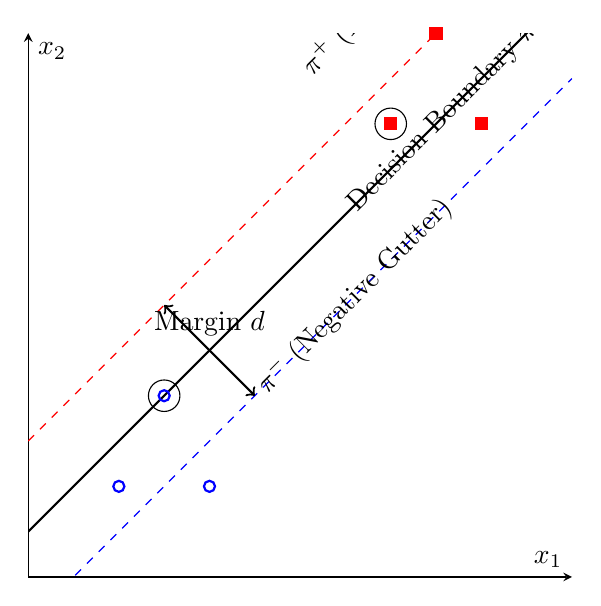
\begin{tikzpicture}
    \begin{axis}[
        xlabel={$x_1$}, ylabel={$x_2$},
        axis lines=middle,
        xmin=0, xmax=6, ymin=0, ymax=6,
        width=0.7\textwidth, height=0.7\textwidth,
        ticks=none
    ]
    % Data Points
    \addplot[only marks, mark=o, color=blue, thick] coordinates {(1,1) (2,1) (1.5,2)};
    \addplot[only marks, mark=square*, color=red, thick] coordinates {(4,5) (5,5) (4.5,6)};
    
    % Support Vectors (Circle them)
    \draw[black, thin] (axis cs:1.5,2) circle(0.2cm);
    \draw[black, thin] (axis cs:4,5) circle(0.2cm);
    
    % Hyperplane (Solid)
    \addplot[domain=0:6, color=black, thick] {x + 0.5};
    \node[right, rotate=45] at (axis cs:3.5, 4) {Decision Boundary $\pi$};
    
    % Margins (Dashed)
    \addplot[domain=0:6, color=blue, dashed] {x + 0.5 - 1.0}; % Shifted down
    \node[right, rotate=45] at (axis cs:2.5, 2) {$\pi^-$ (Negative Gutter)};
    
    \addplot[domain=0:6, color=red, dashed] {x + 0.5 + 1.0}; % Shifted up
    \node[right, rotate=45] at (axis cs:3, 5.5) {$\pi^+$ (Positive Gutter)};
    
    % Margin Arrow
    \draw[<->, thick] (axis cs:2.5, 2) -- (axis cs:1.5, 3);
    \node at (axis cs:2, 2.8) {Margin $d$};
    
    \end{axis}
\end{tikzpicture}
\caption{The Street (Margin). The algorithm pushes the dashed lines as far apart as possible until they hit the data points.}
\label{fig:svm_margin}
\end{figure}

\section{Core Terminology}
This geometry gives rise to three key definitions.

\begin{definition}
\textbf{Hyperplane ($\pi$)}: The decision boundary decision surface. In 2D, it is a line ($w^T x + b = 0$). Ideally, it lies exactly in the middle of the street.
\end{definition}

\begin{definition}
\textbf{Margin ($d$)}: The perpendicular distance between the two marginal planes (the "gutters"). SVM's goal is to \textbf{Maximize} this distance.
\end{definition}

\begin{definition}
\textbf{Support Vectors}: The specific data points that lie exactly on the edge of the margin. They "support" or "hold" the street in place.
\end{definition}

\textbf{Why is this called ``Support Vector Machine''?}
\\ Because the entire model is defined \textit{only} by these Support Vectors.
\\ If you delete the 99\% of data points that are far away from the road, the road does not move. The non-support vectors are mathematically irrelevant. This makes SVM distinct from Logistic Regression (which is affected by all points).

\section{Implementation in Python}
\begin{lstlisting}[language=Python, caption=Basic SVM Classifier]
from sklearn.svm import SVC
from sklearn.datasets import make_blobs
from sklearn.model_selection import train_test_split
from sklearn.preprocessing import StandardScaler

# Generate sample data
X, y = make_blobs(n_samples=100, centers=2, random_state=42)

# Scale features (important for SVM)
scaler = StandardScaler()
X_scaled = scaler.fit_transform(X)

# Train SVM
svm = SVC(kernel='linear', C=1.0)
svm.fit(X_scaled, y)

print(f"Number of Support Vectors: {len(svm.support_vectors_)}")
print(f"Accuracy: {svm.score(X_scaled, y):.2f}")
\end{lstlisting}

\section{HOTS: Interview Questions}
\textbf{Q1: Why is SVM called a ``Maximum Margin Classifier''?}
\begin{itemize}
    \item Because SVM explicitly tries to find the hyperplane that maximizes the distance (margin) between the decision boundary and the nearest data points (support vectors).
\end{itemize}

\textbf{Q2: How does SVM differ from Logistic Regression?}
\begin{itemize}
    \item Logistic Regression minimizes log-loss and is affected by all data points.
    \item SVM maximizes margin and is affected only by support vectors.
    \item SVM uses Hinge Loss, Logistic Regression uses Log Loss.
\end{itemize}

% ========================================
% SECTION: QUICK REFERENCE
% ========================================
\section{Quick Reference Card}

\begin{center}
\fbox{\parbox{0.9\textwidth}{
\textbf{SVM INTUITION - CHEAT SHEET}
\vspace{0.3cm}

\textbf{Core Idea}: Find the ``widest street'' (maximum margin) separating classes

\textbf{Key Components}:
\begin{itemize}
    \item \textbf{Hyperplane}: Decision boundary $w^Tx + b = 0$
    \item \textbf{Margin}: Distance between boundary and nearest points
    \item \textbf{Support Vectors}: Points on the margin edge (the VIPs)
\end{itemize}

\textbf{Margin Width}: $\frac{2}{||w||}$ (maximize by minimizing $||w||$)

\textbf{SVM vs Logistic Regression}:
\begin{center}
\begin{tabular}{|l|l|l|}
\hline
& \textbf{SVM} & \textbf{LogReg} \\ \hline
Loss & Hinge & Log \\ \hline
Points Used & Support Vectors only & All \\ \hline
Goal & Max Margin & Min Log-Loss \\ \hline
\end{tabular}
\end{center}

\textbf{Sklearn}: \texttt{SVC(kernel='linear', C=1.0)}

\textbf{Interview Gold}:
\begin{itemize}
    \item Only support vectors affect the decision
    \item MUST scale features (distance-based)
    \item C controls margin width vs errors tradeoff
\end{itemize}
}}

\chapter{The Curse of Dimensionality}

KNN works beautifully in 2D or 3D. But what happens when we have 1,000 features?
It breaks. This phenomenon is known as the \textbf{Curse of Dimensionality}.

\section{The Concept}
As the number of dimensions ($D$) increases, the volume of the space increases \textbf{exponentially}.
To maintain the same density of data (i.e., to find a neighbor "nearby"), the amount of data needed grows exponentially.

\begin{itemize}
    \item \textbf{1D (Line)}: To cover a unit line with distance 0.1, you need 10 points.
    \item \textbf{2D (Square)}: You need $10^2 = 100$ points.
    \item \textbf{3D (Cube)}: You need $10^3 = 1000$ points.
    \item \textbf{100D (Hypercube)}: You need $10^{100}$ points (More than atoms in the universe).
\end{itemize}

\section{The Sparsity Problem}
In high dimensions, data becomes extremely \textbf{Sparse}. Most of the space is empty.
This means that for any given query point, its "nearest" neighbor is actually \textbf{very far away}.
The concept of "local similarity" breaks down because nothing is local anymore.

\section{Distance Concentration}
In high dimensions, the distance between the nearest point and the farthest point becomes negligible.
\[ \lim_{d \to \infty} \frac{\text{dist}_{max} - \text{dist}_{min}}{\text{dist}_{min}} \to 0 \]
Mathematically, all points become roughly \textbf{equidistant} from each other. If all distances are similar, KNN's voting mechanism becomes random guessing.

\section{Comparison: Lazy vs Eager}
KNN's laziness is a liability here.
\begin{itemize}
    \item \textbf{Eager Learners (SVM, Decision Trees)}: Try to find a separator (hyperplane) that works regardless of the vast empty space. They cope better.
    \item \textbf{Lazy Learners (KNN)}: Rely on finding neighbors in the void. They fail.
\end{itemize}

\section{Solution}
Before using KNN on high-dimensional data (e.g., Images), you must perform \textbf{Dimensionality Reduction}:
\begin{enumerate}
    \item \textbf{PCA (Principal Component Analysis)}: Compress features into simpler components.
    \item \textbf{t-SNE / UMAP}: Manifold learning for visualization.
\end{enumerate}

\section{Interview Questions}

\begin{enumerate}
    \item \textbf{Explain the Curse of Dimensionality to a 5-year-old.}
    \newline \textit{Answer:} Imagine trying to find your friend in a small room. Easy. Now imagine trying to find them in a giant castle with 1000 floors and 1000 rooms per floor. It's empty and lonely, and everyone is far away.
    
    \item \textbf{Why does Euclidean Distance fail in high dimensions?}
    \newline \textit{Answer:} Because of the way high-dimensional geometry works, points tend to concentrate in the corners of the hypercube. The ratio of the volume of an inscribed hypersphere to the hypercube approaches zero. This essentially makes all pairwise distances converge to a constant value.
\end{enumerate}


\part{Naive Bayes}
\chapter{Probability Foundations}

\begin{quote}
    "Probability is the logic of science." — E.T. Jaynes
\end{quote}

Before understanding Naive Bayes, we must master the language of Uncertainty: Probability.

\section{Conditional Probability}
What is the probability of Event A happening \textbf{given that} Event B has already occurred?
\[ P(A|B) = \frac{P(A \cap B)}{P(B)} \]
We restrict our "Universe" to only cases where B happened.

\section{Bayes' Theorem}
This is the Holy Grail of Probabilistic Machine Learning. It flips conditional probabilities:
\[ P(A|B) = \frac{P(B|A) \cdot P(A)}{P(B)} \]

\subsection{Terminology (Important)}
\begin{itemize}
    \item \textbf{$P(A|B)$ - Posterior}: The probability of the hypothesis A being true given the data B. (This is what we want).
    \item \textbf{$P(B|A)$ - Likelihood}: The probability of seeing data B given hypothesis A is true.
    \item \textbf{$P(A)$ - Prior}: The general probability of hypothesis A being true (before seeing data).
    \item \textbf{$P(B)$ - Evidence}: The probability of data B occurring.
\end{itemize}

\section{The Medical Test Paradox}
Why Priors matter.
\begin{itemize}
    \item \textbf{Scenario}: A disease affects 1\% of people ($P(D)=0.01$). A test is 99\% accurate ($P(Pos|D)=0.99$).
    \item \textbf{Question}: You test positive. What is the chance you have the disease?
    \item \textbf{Answer}: It is NOT 99\%. It is roughly \textbf{50\%}.
\end{itemize}

\textbf{Derivation}:
\[ P(D|Pos) = \frac{P(Pos|D)P(D)}{P(Pos)} = \frac{0.99 \times 0.01}{(0.99 \times 0.01) + (0.01 \times 0.99)} = \frac{0.0099}{0.0198} = 0.5 \]

Using Bayes' Theorem helps us avoid this "Base Rate Fallacy". Naive Bayes uses this exact logic to predict classes.

\chapter{Naive Bayes Algorithms}

\section{The "Naive" Assumption}
Calculating the full joint probability $P(x_1, x_2, ..., x_n | y)$ is computationally impossible because it requires a table for every possible combination of features.

To solve this, we make a \textbf{Naive Assumption}:
\begin{quote}
    \textbf{All features are conditionally independent given the class likelihood.}
\end{quote}
\[ P(y|X) \propto P(y) \times \prod_{i=1}^{n} P(x_i | y) \]
This turns a complex $O(2^n)$ problem into a simple $O(n)$ multiplication.

\section{Laplace Smoothing}
What if a word (e.g., "Covid") never appears in the "Spam" dataset during training?
$P(\text{"Covid"} | \text{Spam}) = 0$.
Since we multiply probabilities, the entire prediction becomes 0.

\textbf{Solution}: Add a small constant $\alpha$ (usually 1) to all counts.
\[ P(x_i|y) = \frac{\text{count}(x_i, y) + 1}{\text{count}(y) + N} \]
This ensures no probability is ever exactly zero.

\section{Variants of Naive Bayes}

\subsection{1. Gaussian NB}
Used for \textbf{Numerical Data} (e.g., Age, Salary).
It assumes features follow a Normal (Bell Curve) distribution. It uses the PDF to calculate likelihood:
\[ P(x|y) = \frac{1}{\sqrt{2\pi\sigma^2}} \exp({-\frac{(x-\mu)^2}{2\sigma^2}}) \]

\subsection{2. Multinomial NB}
Used for \textbf{Discrete Counts} (e.g., Text Classification).
It works well when features represent frequency counts (e.g., "Word Count" in an email).

\subsection{3. Bernoulli NB}
Used for \textbf{Binary Features} (e.g., True/False).
It checks only for the \textit{presence} or \textit{absence} of a feature, ignoring frequency.

\section{Interview Questions}

\begin{enumerate}
    \item \textbf{Why is Naive Bayes called "Naive"?}
    \newline \textit{Answer:} Because it assumes features are independent, which is rarely true in the real world (e.g., "Salary" and "Age" are correlated). However, it works efficiently despite this flaw.
    
    \item \textbf{What is the Zero Frequency Problem?}
    \newline \textit{Answer:} If a categorical value appears in the test set but not in the training set, its likelihood is 0, killing the entire prediction. Laplace Smoothing fixes this.
\end{enumerate}


\end{document}
